\begin{figure*}[t]
  \centering
  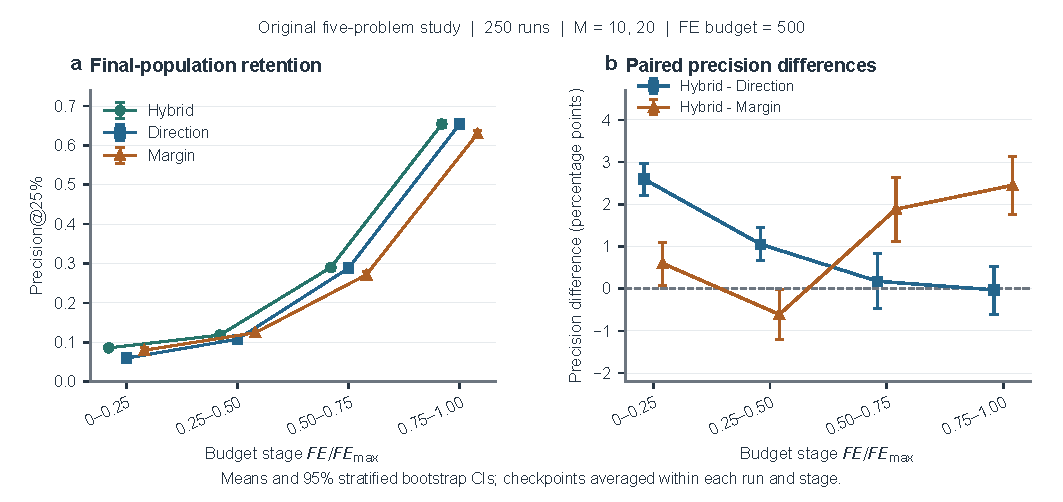
\includegraphics[width=0.98\textwidth]{figures/fig_group_evidence.pdf}
  \caption{Positive-group association with final-population retention in the
  original five-problem study. (a)~Precision of the top-quarter groups.
  (b)~Paired differences between Hybrid and each single-view comparator on the
  same recorded trajectory. Each stage contains 250 run-level values from
  DTLZ2, DTLZ4, DTLZ7, WFG3 and WFG7 at $M=10,20$, with 25 runs per
  configuration and $FE_{\max}=500$. Checkpoints are first averaged within
  run and stage; configurations and runs receive equal weight. Error bars are
  95\% percentile bootstrap confidence intervals from 4,000 resamples of whole
  paired runs within each configuration. Margin denotes the continuous
  representative-margin comparator. These are retention associations along
  recorded Hybrid trajectories.
  \label{fig:group-evidence}}
\end{figure*}
